\RequirePackage[l2tabu,orthodox]{nag}
\documentclass[11pt,letterpaper]{article}
\usepackage[T1]{fontenc}
\usepackage[utf8]{inputenc}
\usepackage{crimson}
\usepackage{helvet}
\usepackage[strict,autostyle]{csquotes}
\usepackage[USenglish]{babel}
\usepackage{microtype}
\usepackage{authblk}
\usepackage{booktabs}
\usepackage{caption}
\usepackage{endnotes}
\usepackage{geometry}
\usepackage{graphicx}
\usepackage{hyperref}
\usepackage{natbib}
\usepackage{rotating}
\usepackage{setspace}
\usepackage{titlesec}
\usepackage{url}
\usepackage{hyperref}
\usepackage{soul}
\usepackage[dvipsnames]{xcolor}
\usepackage[many]{tcolorbox}
\newtcolorbox{mybox}{colback = black!5!gray!50, colframe = black!75!black, segmentation style={solid}} % create text box
\usepackage{hanging}

% location of figure files, via graphicx package
\graphicspath{{./figures/}}

% configure the page layout, via geometry package
\geometry{
	paper=letterpaper,
	top=2.5cm,
	bottom=2.5cm,
	left=2.5cm,
	right=2.5cm}
\setstretch{1.02}
\clubpenalty=10000
\widowpenalty=10000

% set section/subsection headings as the sans serif font
\titleformat{\section}{\normalfont\sffamily\large\bfseries}{\thesection.}{0.3em}{}
\titleformat{\subsection}{\normalfont\sffamily\small\bfseries}{\thesubsection.}{0.3em}{}

% make figure/table captions sans-serif small font
\captionsetup{font={footnotesize,sf},labelfont=bf,labelsep=period}

% configure pdf metadata and link handling
\hypersetup{
	pdfauthor={Carmen Cabrera-Arnau},
	pdftitle={The influence of socioeconomic deprivation on the recovery of urban mobility after COVID-19 in Latin America},
	pdfsubject={Title},
	pdfkeywords={Keywords},
	pdffitwindow=true,
	breaklinks=true,
	colorlinks=false,
	pdfborder={0 0 0}}

\title{The influence of socioeconomic deprivation on the recovery of urban mobility after COVID-19 in Latin America}
\author[1]{Carmen Cabrera-Arnau \thanks{\textit{Corresponding author}: c.cabrera-arnau@liverpool.ac.uk}}
\author[2]{Miguel González-Leonardo}
\author[1]{Andrea Nasuto}
\author[1]{Ruth Neville}
\author[1]{Francisco Rowe}
\affil[1]{Geographic Data Science Lab, Department of Geography and Planning, University of Liverpool, Liverpool, United Kingdom}
\affil[2]{Center for Demographic, Urban and Environmental Studies, El Colegio de México (COLMEX), Mexico City, Mexico}

\date{}

% From pandoc:
% https://github.com/jgm/pandoc-templates/blob/master/default.latex
\newlength{\cslhangindent}
\setlength{\cslhangindent}{1.5em}
\newlength{\csllabelwidth}
\setlength{\csllabelwidth}{3em}
\newlength{\cslentryspacingunit} % times entry-spacing
\setlength{\cslentryspacingunit}{\parskip}
\newenvironment{CSLReferences}[2] % #1 hanging-ident, #2 entry spacing
 {% don't indent paragraphs
  \setlength{\parindent}{0pt}
  % turn on hanging indent if param 1 is 1
  \ifodd #1
  \let\oldpar\par
  \def\par{\hangindent=\cslhangindent\oldpar}
  \fi
  % set entry spacing
  \setlength{\parskip}{#2\cslentryspacingunit}
 }%
 {}
\usepackage{calc}
\newcommand{\CSLBlock}[1]{#1\hfill\break}
\newcommand{\CSLLeftMargin}[1]{\parbox[t]{\csllabelwidth}{#1}}
\newcommand{\CSLRightInline}[1]{\parbox[t]{\linewidth - \csllabelwidth}{#1}\break}
\newcommand{\CSLIndent}[1]{\hspace{\cslhangindent}#1}
\setlength{\emergencystretch}{3em} % prevent overfull lines
\providecommand{\tightlist}{%
  \setlength{\itemsep}{0pt}\setlength{\parskip}{0pt}}

% https://stackoverflow.com/questions/41052687/rstudio-pdf-knit-fails-with-environment-shaded-undefined-error


\begin{document}

\maketitle


\begin{abstract}



%\vspace{1cm}
\end{abstract}



\pagebreak

\section{Introduction}

The COVID-19 pandemic globally resulted in disruptive shocks to the
human mobility system. Governments stringency measures and the economic
downturn caused by the pandemic constrained international migration
({``International Migration 2020: Highlights''} 2021; González-Leonardo
and Spijker 2022; González-Leonardo et al. 2023) and population
movements within countries (Nouvellet et al. 2021; González-Leonardo,
Rowe, and Fresolone-Caparrós 2022; Wang et al. 2022; Rowe,
González-Leonardo, and Champion 2023). During early stages of the
pandemic, big cities became the main epicentres of COVID-19 infections
and deaths (Pomeroy and Chiney 2021) due to their higher connectivity
via air travel, higher population density and concentration of
public-facing jobs (Brandén et al. 2020; Bhadra, Mukherjee, and Sarkar
2020). As a result, governments implemented non-pharmaceutical
interventions, such as lockdowns and business closures, leading to
increases in unemployment and removing the urban vibrancy (Blustein et
al. 2020; BBC news 2023). In addition, remote work and online teaching
reduced the need for commuting, living close to work and education
centers, and added pressure for individuals living in small and crowded
spaces to move out of cities and look for more affordable and
comfortable housing (Nathan and Overman 2020; US Bureau of Labor
Statistics 2021). These changes are believed to have reduced the
attractiveness of cities during the pandemic, while suburbs and rural
areas have gained popularity (Florida, Rodríguez-Pose, and Storper
2021). As a result, a number of headlines have claimed the emergence of
an `urban exodus' to areas with lower population densities (e.g. (The
Guardian 2020)).

Despite their potential rise in popularity, remote locations offer
limited availability and diversity of job opportunities, and tend to
lack infrastructure and services, such as schooling and health, to
effectively accommodate a large population influx (Pinilla and Sáez
2021; \emph{OECD Regions and Cities at a Glance}, n.d.). They generally
lack high-speed Internet connection which is vital for teleworking (Chen
and Wellman 2004). Additionally, most jobs cannot be done remotely
{``OECD Social, Employment and Migration Working Papers''} (n.d.), and
some companies have returned to in-person office work or have
implemented hybrid forms of work, following the relaxation of stringency
measures (McKinsey \& Company 2021). Schools and universities have also
returned to face-to-face teaching. Therefore, living close to work or
study places remains relevant. Businesses and leisure activities in
cities have gradually returned to normal, reinvigorating the economic
functioning and urban life. Collectively, these arguments suggest that a
potential increase in counterurbanisation movements during the pandemic
was concentrated during periods of stringency measures and is likely to
be short term. Big cities have successfully weathered previous pandemics
(Huremović 2019; Glaeser 2020) and are likely to remain attractive
places to live. Thanks to agglomeration economies, cities are normally
regarded as centres for economic growth, clusters of talent, consumer
bases and spaces for face‐to‐face interaction and diversity (Storper and
Venables 2004; Florida, Rodríguez-Pose, and Storper 2021).

Recent empirical evidence has shown a decline on human mobility during
periods of severe stringency measures, coupled with a rise of movements
from cities to less populated areas and a slowdown of urbanisation
movements across some countries of the Global North: the United States
(Ramani and Bloom 2021), United Kingdom (Rowe, González-Leonardo, and
Champion 2023; Wang et al. 2022), Spain (González-Leonardo et al. 2022;
González-Leonardo, Rowe, and Fresolone-Caparrós 2022), Germany {[}@;
Stawarz et al. (2022){]}, Sweden (Vogiazides and Kawalerowicz 2022),
Norway (Tønnessen 2021), Australia (Perales and Bernard 2022) and Japan
Kotsubo and Nakaya (2022). The majority of movements away from cities
headed to their suburbs (Vogiazides and Kawalerowicz 2022; Stawarz et
al. 2022) or rural areas in their close proximity (González-Leonardo et
al. 2022; González-Leonardo, Rowe, and Fresolone-Caparrós 2022) showing
in some instances a ``doghnut effect'', with a decline in population
movements directed to cities and a rise in the inflow of people to less
dense surrounding areas (Ramani and Bloom 2021). Studies demonstrated
that professionals (Tønnessen 2021) and individuals with a high income
(Haslag and Weagley 2021), those who are potentially able to practice
remote working, underpinned movements away from large cities. In
addition, research has shown that a large share of counterurbanisation
movements is headed to touristic locations with a high concentration of
second homes, suggesting that middle and high class individuals may have
been key actors in movements from cities to less populated areas during
the pandemic (González-Leonardo, Rowe, and Fresolone-Caparrós 2022).
However, most studies suggested that variations in internal population
movements during the pandemic are likely to be temporary and have not
altered previous macro-structures of human mobility across the
rural-urban hierarchy (Rowe, González-Leonardo, and Champion 2023).

In Latin America and the Caribbean, a reduction in internal population
movements was documented during periods of high stringency (Aromí et al.
2023), but there is no evidence on how human mobility has changed across
the rural-urban continuum. Anecdotal reports have shown that movements
away from cities seem to have accelerated in two countries of the Global
South, India (Irudaya Rajan, Sivakumar, and Srinivasan 2020) and South
Africa (Ginsburg et al. 2022), while urbanisation trends have
decelerated. However, lack of suitable up-to-date data has prevented us
from properly assessing the ``urban exodus'' hypothesis in Global South
countries, as well as the extent, spatial patterns, and durability of
potential changes on internal population movements. The evidence for
these two countries suggested that increasing counterurbanisation
movements during the pandemic in India and South Africa could be
underpinned by internal migrants residing in cities who returned to
their hometowns due to a rise in unemployment (Irudaya Rajan, Sivakumar,
and Srinivasan 2020; Ginsburg et al. 2022). However, recent studies have
shown that urban residents from wealthy neighborhoods were more likely
to move to rural areas than those from low income neighborhoods during
the first wave of the pandemic in Brazil, Colombia, Mexico, Indonesia,
Philippines and South Africa (Lucchini et al. 2023).

It is known that human mobility within countries tends to vary in
systematic ways with development levels (Bell et al. 2015). In Latin
America and the Caribbean, 28.6\% of the population was living on less
than \$6.8 per day in 2020 (World Bank" 2023) and the informality rate
was about 53\% in 2016 (Salazar-Xirinachs 2018). Thus, we could expect
different pandemic impacts on the patterns of internal population
movements between countries in the Global North and the Global South.
The way in which COVID-19 unfolded in each country, with varying levels
of stringency measures, may have also produced different outcomes on
human mobility.

Traditionally, censuses have been used to analyse human mobility
patterns within Global South countries, which lack register data (Bell
et al. 2015; Bernard et al. 2017). Censuses, however, are normally
updated every 10 years, lacking the temporal granularity to explore
population movements over yearly, monthly or short-time intervals.

Digital traces data from mobile phone applications, on the other hand,
provide a unique opportunity to capture internal population movements
with small spatial and temporal granularity in multiple countries
(Green, Pollock, and Rowe 2021; Rowe 2021). Drawing on geographically
granular Meta-Facebook data from March 2020 to March 2022, we aim to
analyse how the pandemic has changed the patterns of human mobility
across the rural-urban hierarchy in four Latin American countries:
Argentina, Chile, Colombia and Mexico. We aim to address the following
research questions: 1) To what extent did people leave cities and move
to less populated areas in these countries? 2) Which are the spatial
patterns of potential changes on internal population movements? 3) How
have the patterns of human mobility changed over the course of the
pandemic? 4) Are potential changes likely to endure the pandemic?

The rest of the paper is structured as follows: \ldots{}

\section{Background}

\subsection{What do we know about internal population movements during the pandemic?}

The COVID-19 pandemic led to an overall decline in human mobility within
countries (Nouvellet et al. 2021). Research has shown that internal
population movements across the rural-urban continuum decreased in the
United States (Ramani and Bloom 2021), several European countries, Japan
and Austria during 2020 (Rowe, González-Leonardo, and Champion 2023).
Declines ranged from 2.5\% in Spain to 8.5\% in Australia. The largest
drops occurred during periods of national lockdowns and the
implementation of other stringency measures, such as mobility
restrictions, work and school closing, while levels of internal
population movements recovered or exceeded pre-pandemic figures when
lockdowns were lifted. Declines were partially attributed to a reduction
in involuntary migration during lockdowns, a loss of labour market
dynamism due to the pandemic, fewer people changing jobs and increasing
remote work (Perales and Bernard 2022).

COVID-19 has also altered patterns of internal population movements
across the rural-urban hierarchy (Rowe et al. 2022). In large metro
areas across the United States, population movements, as well as
households and businesses, shifted from central cities to suburbs and
exurbs during 2020 (Ramani and Bloom 2021). These authors label this
trend as a ``doughnut effect'', reflecting a decrease in population
inflows and activities in city centers and a growth in suburban rings.
They found a sizeable ``doghnut effect'' in large cities, a smaller
effect in medium-sized cities and almost no effect for small cities. A
similar trend was observed in Norway (Tønnessen 2021), Germany (Stawarz
et al. 2022), Sweden (Vogiazides and Kawalerowicz 2022) and Japan
(Fielding and Ishikawa 2021; Kotsubo and Nakaya 2022), where net
migration rates in big cities declined, while population movement to
their suburbs increased. In addition, this trend was accompanied by a
deceleration of urbanisation trends and unusual population gains in
rural areas due to an acceleration in counterurbanisation movements,
mostly in rural locations which are known to be holiday destinations
with a high concentration of second homes and are generally located in
the close proximity to big cities. An increase of counterurbanisation
was the main pandemic outcome on human mobility in Spain
(González-Leonardo et al. 2022; González-Leonardo, Rowe, and
Fresolone-Caparrós 2022), the United Kingdom (Wang et al. 2022; Rowe et
al. 2022) and Australia (Perales and Bernard 2022), where there is no
evidence of a ``doghnut effect'', since substantial variations in
suburbs were not found across these countries.

However, studies suggest that variations are likely to be temporary
(Rowe, González-Leonardo, and Champion 2023). In Spain, the urbanisation
movement returned to pre-pandemic levels when the lockdown ended in
mid-June 2020 (González-Leonardo et al. 2022) and unusually high levels
of counterurbanisation persisted over 2021, although the majority of
movements continued to occur between and within urban areas
(González-Leonardo, Rowe, and Fresolone-Caparrós 2022). In Australia,
the pandemic has caused minor changes in spatial patterns of internal
migration, and its effects were minimal by the end of 2020 (Perales and
Bernard 2022). In the United Kingdom, mobility patterns returned to
those registered prior to the pandemic after the easing of
non-pharmaceutical interventions (Rowe et al. 2022; Wang et al. 2022).
These findings suggest that COVID-19 generated shock waves leading to
temporary changes in the patterns of internal population movement across
the rural-urban continuum, but it has not significantly altered the
prevalent macro-structures of population movement within countries.

Despite some evidence in the Global North, lees is known about the
impact of COVID-19 on human mobility in the Global South countries. In
Latin America and the Caribbean, internal population movements declined
by 10\% during periods of severe stringent measures, from 16-19\% in
Bolivia, Ecuador and Argentina to less than 3\% in Paraguay and
Venezuela (Aromí et al. 2023). However, there is no evidence about
pandemic outcomes on human mobility across the rural-urban continuum. To
date, surveys carried out in India (Irudaya Rajan, Sivakumar, and
Srinivasan 2020) and South Africa (Ginsburg et al. 2022) have shown
anecdotal evidence suggesting that urbanisation trends declined during
the pandemic, while movements from cities to rural areas increased. Both
studies pointed out that a number of rural residents initiating a
migration decreased during 2020 and some labourers in major cities seem
to have returned to their hometowns due to job losses, since stringency
measures have extensively impacted the functioning of the economy
(Ghosh, Seth, and Tiwary 2020). Many internal migrants residing in
Indian cities lost their jobs and were unable to afford basic
necessities (Nair and Verma 2020). Collectively, these findings suggest
that vulnerable populations seem to have played a role in increasing
counterurbanisation movements in Global South countries. However, recent
work has shown that high-wealth groups residing in cities across Mexico,
Colombia, Brazil, Indonesia, Philippines and South Africa were on
average 159\% more likely to have moved to rural area compared to those
of low-wealth groups during early stages of the pandemic (Lucchini et
al. 2023), in line with the evidencee found for Global North countries.

Despite anecdotal evidence suggesting pandemic impacts on the patterns
of human mobility across the rural-urban hierarchy in the Global South,
lack of suitable data has not allowed us to identify and quantify the
magnitude of these impacts. In this paper, we use Meta-Facebook data to
provide evidence on the effect of the pandemic on the patterns of
internal population movements across four Latin American countries.

\subsection{Contemporary trends of human mobility across the rural-urban hierarchy in Latin America}

Until 1980, rural to urban migration dominated internal population
movements in Latin America with significant levels of population
redistribution, especially during the rapid industrialisation process
between the 1950s and 1970s when a critical mass of individuals moved
from villages and towns to urban areas (Firebaugh 1979; A. Lattes 1995;
J. Sobrino 2012). Urban growth due to internal mobility was primarily
concentrated in large urban centres resulting in a significant
population imbalance between the chief cities and other settlements
(Pinto da Cunha 2002; A. E. Lattes, Rodríguez, and Villa 2017). As a
consequence, Latin America shows high rates of urbanisation with more
than 81\% of the population living in cities, the highest figure after
North America, and about 46\% of urban residents settled in cities with
more than 1 million inhabitants (Nations" 2019).

Currently, internal population movements amongst cities dominate the
migratory system in Latin America, while rural to urban flows are of
less importance (Bernard et al. 2017; Rodríguez-Vignoli and Rowe 2018;
Nations" 2019). According to the 2010 census round, 80\% of internal
migrants moved between cities (Rodríguez-Vignoli and Rowe 2018).
Contrary to the period preceding the 1980s, medium-sizes cities (those
between 500K and 1 million inhabitants) experienced the highest net
migration rates, while large cities (\textgreater1 million) presented
balanced rates and small cities (\textgreater500K) lost individuals by
internal population movements (Rodríguez-Vignoli and Rowe 2018).
Changing patterns in human mobility within Latin American countries were
driven by a decline in internal migration since the 1980s crisis (Chávez
Galindo et al. 2016) and deconcentration dynamics in large urban
centres, such as Mexico City (Jaime Sobrino 2006) or Santiago de Chile
(González Ollino and Rodríguez Vignoli 2006), where long distance
inflows have declined over time. At the same time, there has been an
increasing domestic and foreign investment in export-oriented activities
or tourism industries in certain middle-sized cities, fostering the
geographic dispersal of employment opportunities and increasing the
attractiveness of these cities (Brea 2003; Pérez-Campuzano 2013; Chávez
Galindo et al. 2016).

Suburbanisation also represents an important type of internal population
movement and has increased over time due to the growing expansion of
Latin American cities (Graizbord and Acuña 2007; Chávez Galindo et al.
2016). These movements are underpinned by flows of middle- and
upper-class families moving away from central cities to surrounding
auto-segregated areas of wealthy individuals (Borsdorf 2003; Rodríguez
Vignoli and Rowe 2017). Low-income populations also settle in specific
areas within suburbs where the cost of living is usually cheaper than in
cities (Janoschka 2002; Rodríguez Vignoli and Rowe 2017). A large
proportion of both wealthy individuals and low-income residents commute
daily to central cities, mainly for work reasons (Chávez Galindo et al.
2016). Recently, reurbanisation dynamics have also been observed due to
gentrification processes in specific central areas (J. Sobrino 2012;
Chávez Galindo et al. 2016). In this paper, we analyse how the COVID-19
pandemic has changed patterns of internal population movements across
the rural-urban hierarchy in Mexico, Colombia, Perú, Chile and
Argentina.

\section{Data}

The analysis proposed in this paper is based on several data sets.
Firstly, Facebook Population and Facebook Movements are data sets based
on the Facebook users' location history. The data sets were created by
Facebook's owner company Meta and can be accessed through their Data for
Good programme (\url{https://dataforgood.facebook.com/}). Prior to
releasing the data sets, Meta applies three techniques to ensure privacy
and anonymisation. First, a small undisclosed amount of random noise is
added to ensure that precise location cannot be identified for small
population counts in sparsely populated areas. While removing small
counts may lead to an underrepresentation of the population in these
places, the geographic distribution of population is still reflected in
the data. Second, spatial smoothing is applied to produce a smooth
population count surface using inverse distance-weighted averaging.
Third, any remaining population counts of less than 10 are removed from
the final data set (see Maas et al. Maas et al. (2019) for details).

Both data sets Facebook Population and Facebook Movements contain data
corresponding to a time period comprising approximately two years,
starting from March 2020, and to four Latin American countries,
Argentina, Chile, Colombia and Mexico. The data in both data sets is
temporally aggregated into three 8-hour windows (00:00--08:00,
08:00--16:00 and 16:00--00:00) for every day in the aforementioned
two-year period. It is spatially aggregated into tiles according to the
Bing Maps Tile System. This geospatial indexing system was developed by
Microsoft and it partitions the world into square cells at various
levels of resolution. The Facebook Movements and Facebook Population
datasets are aggregated into various levels of resolution depending on
the country, and the length of the Bing tile sides vary also by country
according to the country's distance to the Equator, even when two
countries use tiles at the same level of resolution.

The Facebook Population data set provides information on the number of
active Facebook users in each tile. The data set Facebook Movements
captures the total number of Facebook users moving between pairs of
origin and destination Bing tiles. We note here that due to the nature
of the Facebook Movement data, we cannot distinguish between different
types of movements, for example, daily commutes to work or permanent
changes of address. However, we are still able to detect the evolution
of movements between origin-destination pairs of Bing tiles and hence,
we are able to capture the impact that COVID-19 has on mobility
patterns.

On top of the data for the two-year period, each entry in the Facebook
Population and Facebook Movements datasets include data for baseline
levels before COVID-19. The baseline values are computed based on a
45-day period ending on the 10th of March of 2020. The data sets also
include a `quality' score indicating the number of standard deviations
by which the observed data at specific locations and time windows differ
from the baseline values, hence highlighting statistically significant
changes.

An additional data set from WorldPop was used to capture the spatial
distribution of population density in the different countries analysed
here. The WorlPop dataset is in raster format and contains gridded
population data at 1 sqkm resolution.

\section{Method}

\subsection{Data pre-processing}

Ultimately, we work with a dataset where each entry represents a
population flow between an origin and a destination pair. For each
entry, we consider when the movement took place, the population density
at the origin and destination, the number of active Facebook users at
the origin and destination and?

\subsubsection{Spatial aggregation}

The working dataset is aggregated at the same level as the Bing tiles
used to track the movements in a given country. To each Bing tile, we
aggregate WorldPop population data and use it to estimate the population
density of each Bing tile.

\subsubsection{Temporal aggregation}

The raw data is aggregated into 8-hour windows for every day in the
two-year period. However, we are interested in longer-term trends and
not in how population flows vary throughout the day. For this reason, we
obtain estimates for the parameters in the models described in
subsection \ref{subsec-models} by splitting the total data set by month.
For the visualisations in section \ref{sec-results}, we also present the
data aggregated by month.

\subsection{Classifying Bing tiles according to their population density}

Here we aim to understand how the population density at the origin and
the destination might influence mobility behaviours. To help
characterise the population density between orign and destination, we
classify the Bing tiles into 10 discrete categories of population
density according to the Jenks natural breaks classification method,
hence obtaining a categorisation of Bing tiles a lot more detailed than
the traditional binary rural/urban classification.

\begin{figure}[H]

{\centering 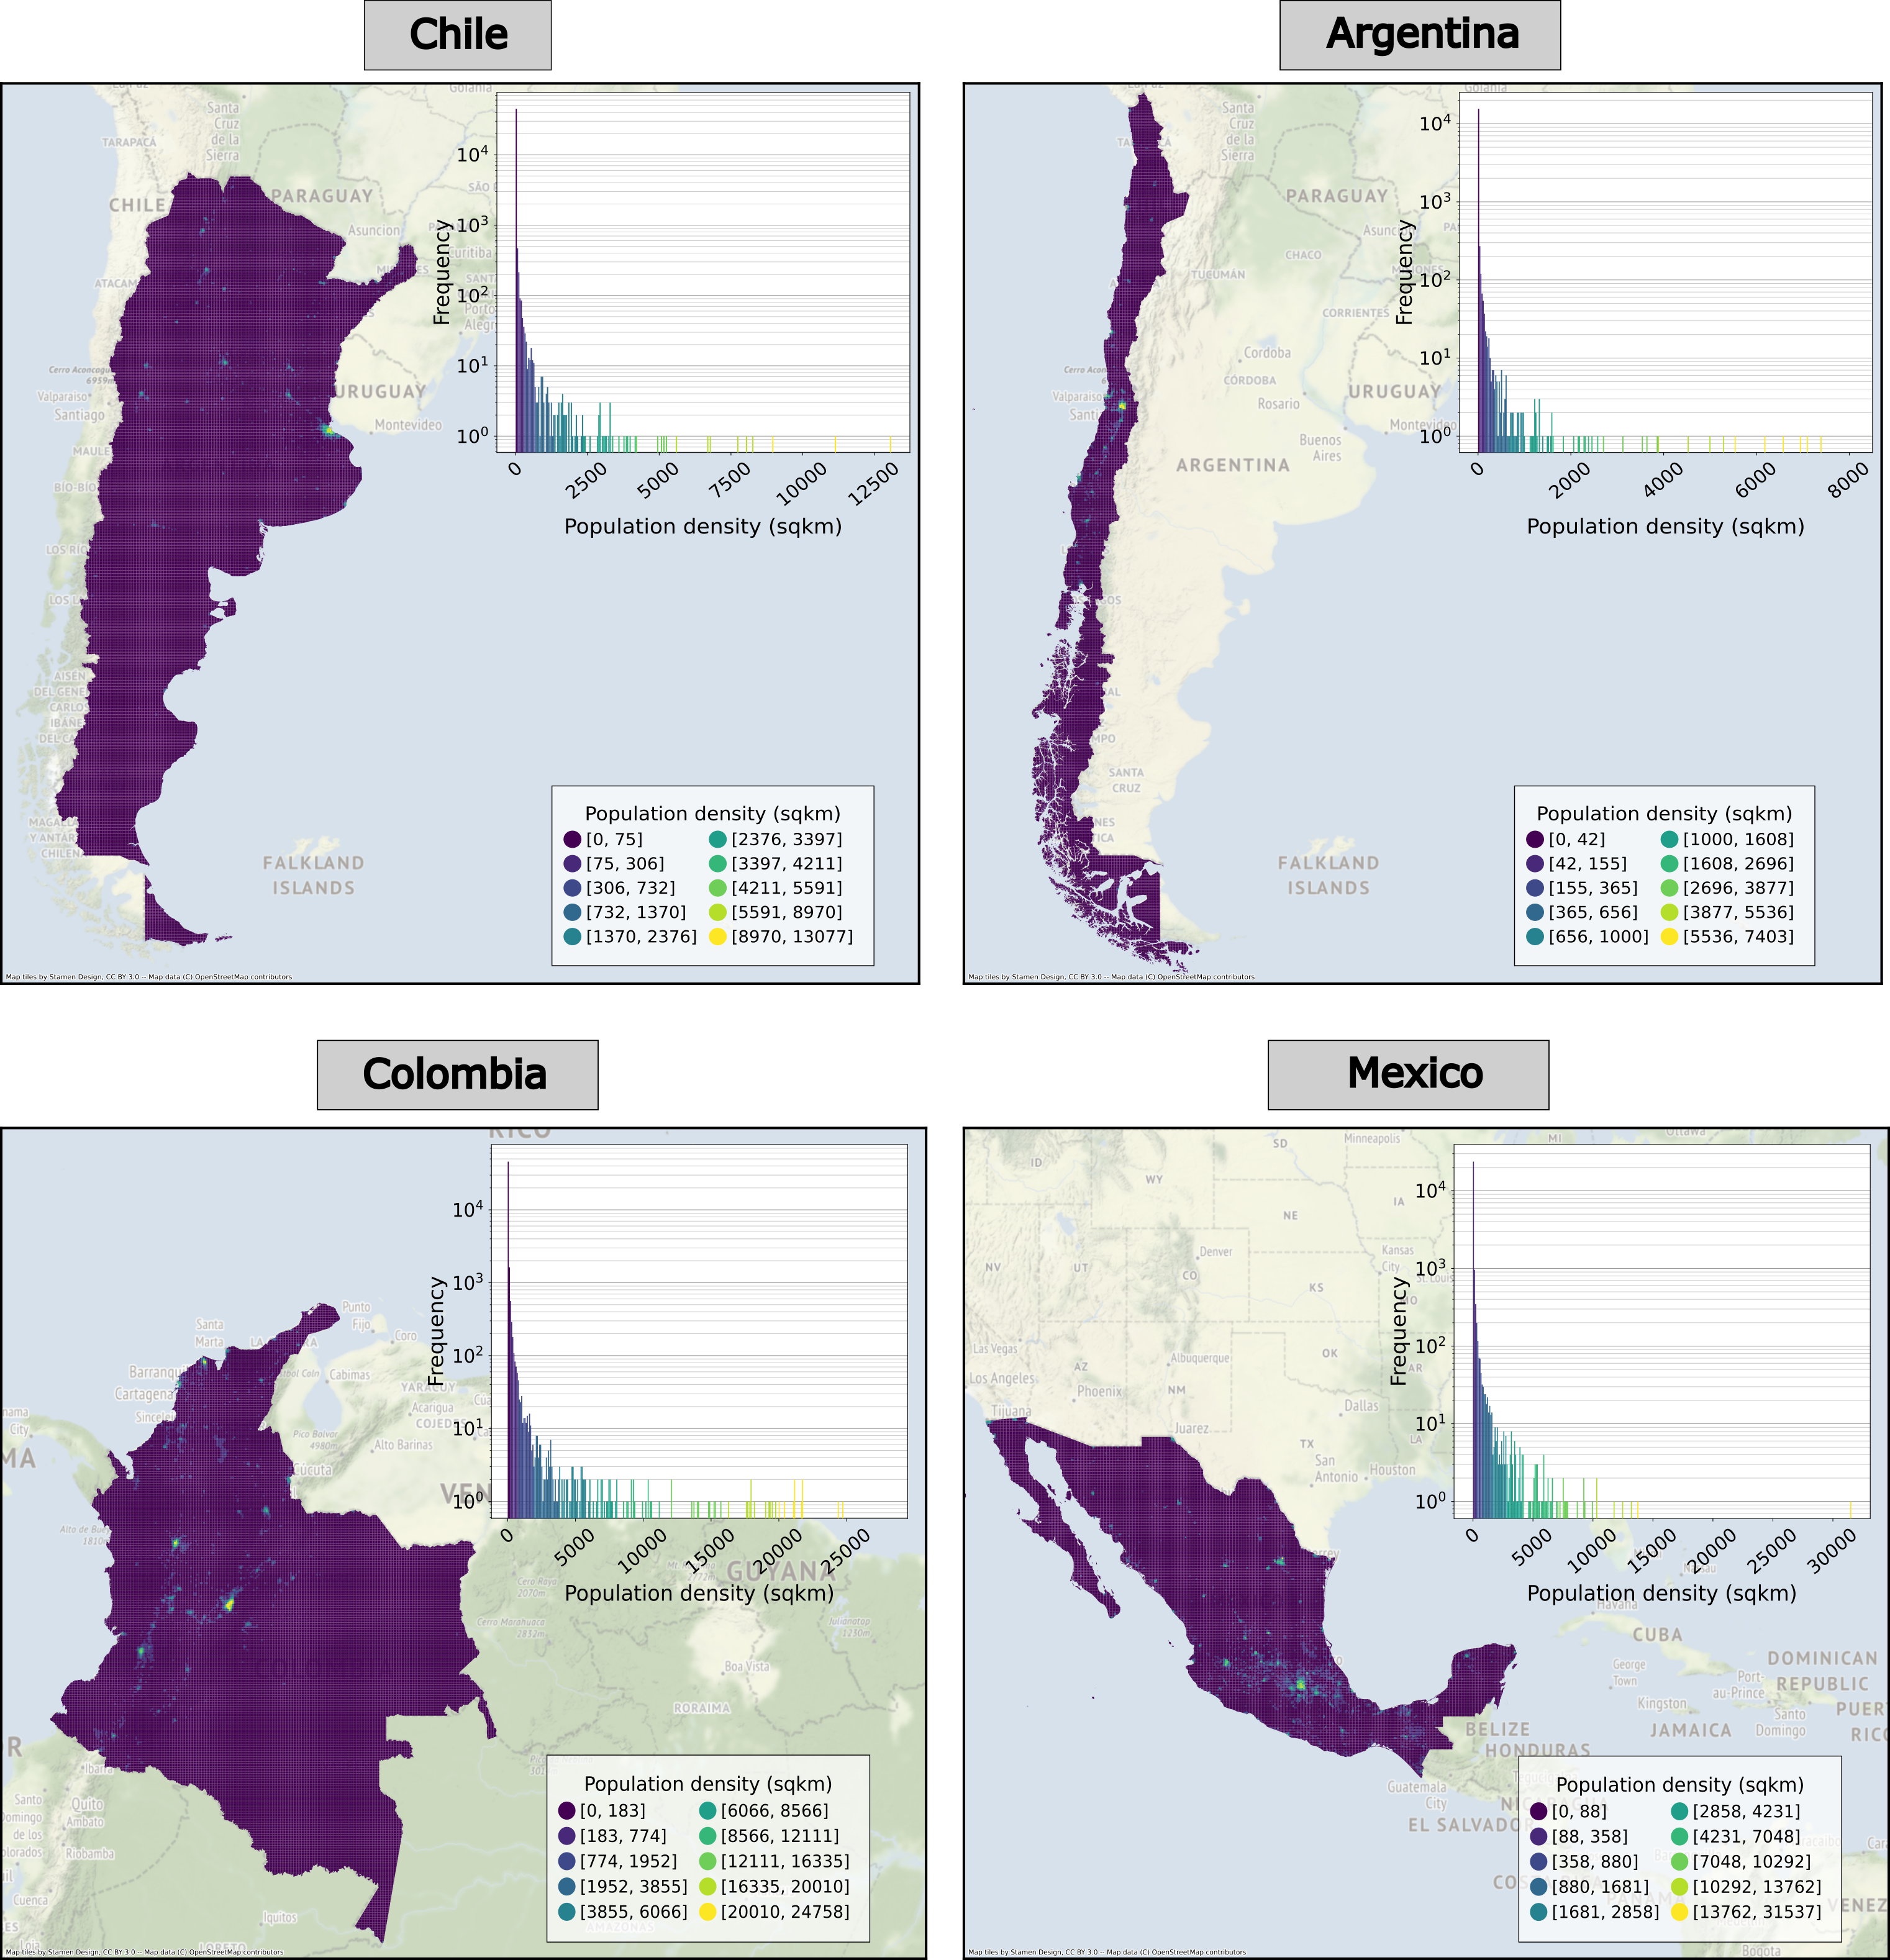
\includegraphics[width=6.51042in,height=6.66667in]{figures/Map_density_histogram.png}

}

\caption{Maps of population density categories by country with
histograms, showing that the distribution of Bing tiles in each density
category.}

\end{figure}%

\subsection{Estimating the strength of the flows between tiles of different population density categories}

\ref{subsec-models}

In this section, we propose a statistical model to capture the extent to
which the strength of the population flows is systematically impacted by
the density classes of the origin and destination tiles, and how this
effect varies over time. Our approach here is very similar to that
proposed by \cite{Rowe}.

While we could obtain the population flows between different population
classes and their evolution over time, the results would fail to capture
specifically the effect of the density classes of the origin and
destination tiles. This is due to the fact that movement patterns are
influenced not only by the population density of the starting and ending
locations, but also by factors such as the distance, the population
size, the time of the week and day at which movements take place, etc.
These additional variables can act as confounding factors, obscuring the
actual impact of population density. In order to disentangle and obtain
a more accurate estimation of the importance of population density, we
chose to utilise a regression modeling approach. I AM HERE

We adopted a spatial interaction framework (Rowe, Lovelace, et al.,
2022). We used population flows between tiles by time window and day (as
described in Section 3), and modelled them as a function of
characteristics of the flow itself (Fij), the origin (Tilei) and
destination (Tilej) tiles and the temporal nature of the flow (Tw).
Crucially, we included indicator variables that capture the pair of
population classes (Figure 1) of the origin and destination tile. In
mathematical form:

\begin{enumerate}
\def\labelenumi{(\arabic{enumi})}
\setcounter{enumi}{1}
\tightlist
\item
  where µijw is the expectation of the flow of people from tile i to
  tile j in the time window w; ⍺ is an intercept; is a series of
  indicator variables that reflect the pair of population density
  classes of a given origin i (I) and destination tile j (J), resulting
  in 99 pairs (10 classes × 10 classes minus one so it is not collinear
  with ⍺); dij is the geographic distance between tiles i and j; qijw is
  a measure of the quality of the flow estimate provided by
  Meta-Facebook and related to the uncertainty behind the user count of
  the flow as described in Section 3; Popi,j represents the population
  at the origin (i) and destination (j) tiles; are parameters to
  estimate in the model linking their respective covariates to µijw; D
  is a trend tracking the day to which the flow relates to during the
  period in analysis; while Wk and H are indicator variables capturing
  day of the week (i.e., weekday or weekend) and hour window (i.e.,
  00:00--08:00, 08:00--16:00 and 16:00--00:00). Our focus in Equation
  (2) is centred on . Controlling for all other variables, these
  parameters capture the extent to which, the expected flow between a
  given origin-destination population density class pair of tiles (e.g.,
  a high-density origin to a low-density destination) is systematically
  higher or lower than if it occurred between a baseline
  origin-destination population density class pair of tiles (e.g., a
  low-density origin to a low-density destination). Additionally, we
  standardised continuous variables (dij, qijw, Popi j), α so that they
  can be interpreted as the expected flow on the first day (D = 0),
  during the first temporal window (H = 00:00--08:00), on a weekday
  (Wk = 0), for the baseline origin-population population density class
  pair, when all the other variables are at their mean value. In this
  context, each can also be seen as the `modulation factor' around that
  expectation associated with each pair of origin-destination classes.
  The baseline origin-destination population density class pair is the
  lowest population density class as origin and destination.
\end{enumerate}

We used a count data regression model. Specifically, we fitted a
generalised linear model (GLM) where the error term is assumed to be
distributed following a Poisson distribution, with a flow expectation of
(µijw) linked to the flow count (Fijw) through a log link: (3) (4) The
Poisson regression model (PRM) assumes that equidispersion, that is,
equality of mean and variance in the response variable (Cameron \&
Trivedi, 2013). In practice, the equidispersion property is commonly
violated because of overdispersion, that is, the variance exceeds the
mean. When this occurs, the PRM may produce biased parameter estimates,
causing the standard errors of the estimates to be underestimated, and
compromising the statistical inference process (Hilbe, 2011). To test
for overdispersion, we used a regression-based test based on an
auxiliary regression of the conditional variance as described in Cameron
and Trivedi (2013).

Following Gelman and Hill (2006), we used a quasi-PRM to address
overdispersion in our response variable. This is one of the most common
strategies to deal with overdispersion in count data models (Hilbe,
2011). Intuitively, this model adjusts the standard errors of the
estimates to account for the extra dispersion in the data. To implement
this, we estimated Equation (2) by using robust variance estimators. The
number of active Facebook users were used as a weight to account for the
variability of the observed count of population movement over time. This
strategy is also used to mitigate for any potential biases regarding the
variation in the observed number of active Facebook users changes over
time across Britain.

We fitted Equation (2) using iteratively reweighted least squares
(IWLS). We separately estimated models for individual months in our
data, resulting in 18 sets of estimates. Our key aim was to generate
estimates for ⍺ and , so that we focused on discussing the evolution of
these estimates in a grid of line plots with 10 rows and 10 columns,
each of them representing one of our population density classes. The
plot corresponding to the Ith row and Jth column displays the evolution
of the parameter that tracks the intensity of population flows from
tiles in population density class Ith to those in population density
class Jth.

\section{Results}\label{sec-results}

\section{Discussion}

\section{Conclusion}

\section{References}

\phantomsection\label{refs}
\begin{CSLReferences}{1}{0}
\bibitem[\citeproctext]{ref-aromuxed2023}
Aromí, Daniel, María Paula Bonel, Julian Cristia, Martín Llada, Juan
Pereira, Xiomara Pulido, and Julieth Santamaria. 2023. {``\#StayAtHome:
Social Distancing Policies and Mobility in Latin America and the
Caribbean.''} \emph{Economía} 22 (1).
\url{https://doi.org/10.31389/eco.4}.

\bibitem[\citeproctext]{ref-BBCnews2023}
BBC news. 2023. {``Unemployment: Who Are the Millions of Britons Not
Working?''} \url{https://www.bbc.co.uk/news/business-52660591}.

\bibitem[\citeproctext]{ref-bell2015}
Bell, Martin, Elin Charles-Edwards, Philipp Ueffing, John Stillwell,
Marek Kupiszewski, and Dorota Kupiszewska. 2015. {``Internal Migration
and Development: Comparing Migration Intensities Around the World.''}
\emph{Population and Development Review} 41 (1): 33--58.
\url{https://doi.org/10.1111/j.1728-4457.2015.00025.x}.

\bibitem[\citeproctext]{ref-bernard2017}
Bernard, Aude, Francisco Rowe, Martin Bell, Philipp Ueffing, and Elin
Charles-Edwards. 2017. {``Comparing Internal Migration Across the
Countries of Latin America: A Multidimensional Approach.''} Edited by
Osman Alimamy Sankoh. \emph{PLOS ONE} 12 (3): e0173895.
\url{https://doi.org/10.1371/journal.pone.0173895}.

\bibitem[\citeproctext]{ref-bhadra2020}
Bhadra, Arunava, Arindam Mukherjee, and Kabita Sarkar. 2020. {``Impact
of Population Density on Covid-19 Infected and Mortality Rate in
India.''} \emph{Modeling Earth Systems and Environment} 7 (1): 623--29.
\url{https://doi.org/10.1007/s40808-020-00984-7}.

\bibitem[\citeproctext]{ref-blustein2020}
Blustein, David L., Ryan Duffy, Joaquim A. Ferreira, Valerie
Cohen-Scali, Rachel Gali Cinamon, and Blake A. Allan. 2020.
{``Unemployment in the Time of COVID-19: A Research Agenda.''}
\emph{Journal of Vocational Behavior} 119 (June): 103436.
\url{https://doi.org/10.1016/j.jvb.2020.103436}.

\bibitem[\citeproctext]{ref-borsdorf2003}
Borsdorf, Axel. 2003. {``Cómo Modelar El Desarrollo y La Dinámica de La
Ciudad Latinoamericana.''} \emph{EURE (Santiago)} 29 (86).
\url{https://doi.org/10.4067/s0250-71612003008600002}.

\bibitem[\citeproctext]{ref-branduxe9n2020}
Brandén, Maria, Siddartha Aradhya, Martin Kolk, Juho Härkönen, Sven
Drefahl, Bo Malmberg, Mikael Rostila, Agneta Cederström, Gunnar
Andersson, and Eleonora Mussino. 2020. {``Residential Context and
COVID-19 Mortality Among Adults Aged 70 Years and Older in Stockholm: A
Population-Based, Observational Study Using Individual-Level Data.''}
\emph{The Lancet Healthy Longevity} 1 (2): e80--88.
\url{https://doi.org/10.1016/s2666-7568(20)30016-7}.

\bibitem[\citeproctext]{ref-Brea03}
Brea, J. 2003. {``Population Dynamics in Latin America.''}
\emph{Population Bulletin} 58: 3--36.
\url{https://population.un.org/wup/Publications/Files/WUP2018-Report.pdf}.

\bibitem[\citeproctext]{ref-chuxe1vezgalindo2016}
Chávez Galindo, Ana María, Jorge Rodríguez Vignoli, Mario Acuña, Jorge
Barquero, Daniel Macadar, José Marcos Pinto da Cunha, and Jaime Sobrino.
2016. {``Migración Interna y Cambios Metropolitanos.''} \emph{Revista
Latinoamericana de Población} 10 (18): 7--41.
\url{https://doi.org/10.31406/relap2016.v10.i1.n18.1}.

\bibitem[\citeproctext]{ref-Chen2004}
Chen, Wenhong, and Barry Wellman. 2004. {``The Global Digital Divide -
Within and Between Countries.''} \emph{IT \& Society} 1: 39--45.
\url{http://www.ifs.tuwien.ac.at/~dieter/teaching/GmA/Chen2004.pdf}.

\bibitem[\citeproctext]{ref-fielding2021}
Fielding, Tony, and Yoshitaka Ishikawa. 2021. {``COVID{-}19 and
Migration: A Research Note on the Effects of COVID{-}19 on Internal
Migration Rates and Patterns in Japan.''} \emph{Population, Space and
Place} 27 (6). \url{https://doi.org/10.1002/psp.2499}.

\bibitem[\citeproctext]{ref-firebaugh1979}
Firebaugh, Glenn. 1979. {``Structural Determinants of Urbanization in
Asia and Latin America, 1950- 1970.''} \emph{American Sociological
Review} 44 (2): 199. \url{https://doi.org/10.2307/2094505}.

\bibitem[\citeproctext]{ref-florida2021}
Florida, Richard, Andrés Rodríguez-Pose, and Michael Storper. 2021.
{``Critical Commentary: Cities in a Post-COVID World.''} \emph{Urban
Studies} 60 (8): 1509--31.
\url{https://doi.org/10.1177/00420980211018072}.

\bibitem[\citeproctext]{ref-ghosh2020}
Ghosh, Somenath, Pallabi Seth, and Harsha Tiwary. 2020. {``How Does
Covid-19 Aggravate the Multidimensional Vulnerability of Slums in India?
A Commentary.''} \emph{Social Sciences \& Humanities Open} 2 (1):
100068. \url{https://doi.org/10.1016/j.ssaho.2020.100068}.

\bibitem[\citeproctext]{ref-ginsburg2022}
Ginsburg, Carren, Mark A. Collinson, F. Xavier Gómez-Olivé, Sadson
Harawa, Chantel F. Pheiffer, and Michael J. White. 2022. {``The Impact
of COVID-19 on a Cohort of Origin Residents and Internal Migrants from
South Africa's Rural Northeast.''} \emph{SSM - Population Health} 17
(March): 101049. \url{https://doi.org/10.1016/j.ssmph.2022.101049}.

\bibitem[\citeproctext]{ref-Glaeser20}
Glaeser, Edward L. 2020. {``Cities and Pandemics Have a Long History.
City Journal.''}
\url{https://www.city-journal.org/article/cities-and-pandemics-have-a-long-history}.

\bibitem[\citeproctext]{ref-gonzuxe1lezollino2006}
González Ollino, Daniela, and Jorge Rodríguez Vignoli. 2006. {``Spatial
Redistribution and Internal Migration of the Populationin Chile over the
Past 35 Years (1965-20).''} \emph{Estudios Demográficos y Urbanos} 21
(2): 369. \url{https://doi.org/10.24201/edu.v21i2.1253}.

\bibitem[\citeproctext]{ref-gonzuxe1lez-leonardo2022b}
González-Leonardo, Miguel, Antonio López-Gay, Niall Newsham, Joaquín
Recaño, and Francisco Rowe. 2022. {``Understanding Patterns of Internal
Migration During the COVID{-}19 Pandemic in Spain.''} \emph{Population,
Space and Place} 28 (6). \url{https://doi.org/10.1002/psp.2578}.

\bibitem[\citeproctext]{ref-gonzuxe1lez-leonardo2023}
González-Leonardo, Miguel, Michaela Potančoková, Dilek Yildiz, and
Francisco Rowe. 2023. {``Quantifying the Impact of COVID-19 on
Immigration in Receiving High-Income Countries.''} Edited by Ricky Chee
Jiun Chia. \emph{PLOS ONE} 18 (1): e0280324.
\url{https://doi.org/10.1371/journal.pone.0280324}.

\bibitem[\citeproctext]{ref-gonzuxe1lez-leonardo2022a}
González-Leonardo, Miguel, Francisco Rowe, and Alberto
Fresolone-Caparrós. 2022. {``Rural Revival? The Rise in Internal
Migration to Rural Areas During the COVID-19 Pandemic. Who Moved and
Where?''} \emph{Journal of Rural Studies} 96 (December): 332--42.
\url{https://doi.org/10.1016/j.jrurstud.2022.11.006}.

\bibitem[\citeproctext]{ref-gonzuxe1lez-leonardo2022}
González-Leonardo, Miguel, and Jeroen Spijker. 2022. {``The Impact of
Covid-19 on Demographic Components in Spain, 2020{\textendash}31: A
Scenario Approach.''} \emph{Population Studies}, November, 1--17.
\url{https://doi.org/10.1080/00324728.2022.2138521}.

\bibitem[\citeproctext]{ref-graizbord2007}
Graizbord, Boris, and Beatriz Acuña. 2007. {``Movilidad Residencial En
La Ciudad de México / Residential Mobility in Mexico City.''}
\emph{Estudios Demográficos y Urbanos} 22 (2): 291.
\url{https://doi.org/10.24201/edu.v22i2.1281}.

\bibitem[\citeproctext]{ref-green2021}
Green, Mark, Frances Darlington Pollock, and Francisco Rowe. 2021.
{``New Forms of Data and New Forms of Opportunities to Monitor and
Tackle a Pandemic.''} In, 423--29. Springer International Publishing.
\url{https://doi.org/10.1007/978-3-030-70179-6_56}.

\bibitem[\citeproctext]{ref-haslag2021}
Haslag, Peter H., and Daniel Weagley. 2021. {``From L.A. To Boise: How
Migration Has Changed During the COVID-19 Pandemic.''} \emph{SSRN
Electronic Journal}. \url{https://doi.org/10.2139/ssrn.3808326}.

\bibitem[\citeproctext]{ref-huremovic2019}
Huremović, Damir. 2019. {``Brief History of Pandemics (Pandemics
Throughout History).''} In, 7--35. Springer International Publishing.
\url{https://doi.org/10.1007/978-3-030-15346-5_2}.

\bibitem[\citeproctext]{ref-internat2021}
{``International Migration 2020: Highlights.''} 2021, January.
\url{https://doi.org/10.18356/9789210052689}.

\bibitem[\citeproctext]{ref-irudayarajan2020}
Irudaya Rajan, S., P. Sivakumar, and Aditya Srinivasan. 2020. {``The
COVID-19 Pandemic and Internal Labour Migration in India: A {`}Crisis of
Mobility{'}.''} \emph{The Indian Journal of Labour Economics} 63 (4):
1021--39. \url{https://doi.org/10.1007/s41027-020-00293-8}.

\bibitem[\citeproctext]{ref-janoschka2002}
Janoschka, Michael. 2002. {``El Nuevo Modelo de La Ciudad
Latinoamericana: Fragmentación y Privatización.''} \emph{EURE
(Santiago)} 28 (85).
\url{https://doi.org/10.4067/s0250-71612002008500002}.

\bibitem[\citeproctext]{ref-kotsubo2022}
Kotsubo, Masaki, and Tomoki Nakaya. 2022. {``Trends in Internal
Migration in Japan, 2012{\textendash}2020: The Impact of the COVID{-}19
Pandemic.''} \emph{Population, Space and Place} 29 (4).
\url{https://doi.org/10.1002/psp.2634}.

\bibitem[\citeproctext]{ref-lattes95}
Lattes, A. 1995. {``Urbanización, Crecimiento Urbano y Migraciones En
América Latina. Población y Desarrollo: Tendencias y Desafíos.''}
\emph{Notas de Población} 62: 211--60.
\url{https://repositorio.cepal.org/handle/11362/38594}.

\bibitem[\citeproctext]{ref-lattes2017}
Lattes, Alfredo E., Jorge Rodríguez, and Miguel Villa. 2017.
{``Population Dynamics and Urbanization in Latin America: Concepts and
Data Limitations.''} In, 89--111. Routledge.
\url{https://doi.org/10.4324/9781315248073-5}.

\bibitem[\citeproctext]{ref-lucchini2023}
Lucchini, Lorenzo, Ollin Langle-Chimal, Lorenzo Candeago, Lucio Melito,
Alex Chunet, Aleister Montfort, Bruno Lepri, Nancy Lozano-Gracia, and
Samuel P. Fraiberger. 2023. {``Socioeconomic Disparities in Mobility
Behavior During the COVID-19 Pandemic in Developing Countries.''}
\url{https://doi.org/10.48550/ARXIV.2305.06888}.

\bibitem[\citeproctext]{ref-Maas19}
Maas, P., S. Iyer, A. Gros, W. Park, L. McGorman, C. Nayak, and P. A.
Dow. 2019. {``Facebook Disaster Maps: Aggregate Insights for Crisis
Response and Recovery.''} In \emph{16th International Conference on
Information Systems for Crisis Response and Management}, 836--47.

\bibitem[\citeproctext]{ref-McKinsey21}
McKinsey \& Company. 2021. {``What Executives Are Saying about the
Future of Hybrid Work.''}
\url{https://www.mckinsey.com/capabilities/people-and-organizational-performance/our-insights/what-executives-are-saying-about-the-future-of-hybrid-work}.

\bibitem[\citeproctext]{ref-ILO2020}
Nair, Shabari, and Divya Verma. 2020. {``A Policy Framework for India's
Covid-19 Migration. International Labour Organization.''}
\url{https://www.ilo.org/newdelhi/info/public/fs/WCMS_746654/lang--en/index.htm}.

\bibitem[\citeproctext]{ref-nathan2020}
Nathan, Max, and Henry Overman. 2020. {``Will Coronavirus Cause a Big
City Exodus?''} \emph{Environment and Planning B: Urban Analytics and
City Science} 47 (9): 1537--42.
\url{https://doi.org/10.1177/2399808320971910}.

\bibitem[\citeproctext]{ref-UNpopulation19}
Nations", "United. 2019. {``World Urbanization Prospects. The 2018
Revision.''}
\url{https://population.un.org/wup/Publications/Files/WUP2018-Report.pdf}.

\bibitem[\citeproctext]{ref-nouvellet2021}
Nouvellet, Pierre, Sangeeta Bhatia, Anne Cori, Kylie E. C. Ainslie, Marc
Baguelin, Samir Bhatt, Adhiratha Boonyasiri, et al. 2021. {``Reduction
in Mobility and COVID-19 Transmission.''} \emph{Nature Communications}
12 (1). \url{https://doi.org/10.1038/s41467-021-21358-2}.

\bibitem[\citeproctext]{ref-oecdreg}
\emph{OECD Regions and Cities at a Glance}. n.d. OECD.
\url{https://doi.org/10.1787/26173212}.

\bibitem[\citeproctext]{ref-oecdsoc}
{``OECD Social, Employment and Migration Working Papers.''} n.d.
\url{https://doi.org/10.1787/1815199x}.

\bibitem[\citeproctext]{ref-perales2022}
Perales, Francisco, and Aude Bernard. 2022. {``Continuity or Change? How
the Onset of COVID{-}19 Affected Internal Migration in Australia.''}
\emph{Population, Space and Place} 29 (2).
\url{https://doi.org/10.1002/psp.2626}.

\bibitem[\citeproctext]{ref-Puxe9rez-Campuzano13}
Pérez-Campuzano, C., E. y Santos-Cerquera. 2013. {``Tendencias Recientes
de La Migración Interna En México.''} \emph{"Papeles de Población"} 19:
53--88.
\url{https://www.scielo.org.mx/scielo.php?script=sci_arttext&pid=S1405-74252013000200003}.

\bibitem[\citeproctext]{ref-Pinilla2021}
Pinilla, Vicente, and Luis Antonio Sáez. 2021. {``La Despoblación Rural
En España: Características, Causas e Implicaciones Para Las Políticas
Públicas.''} \emph{Presupuesto y Gasto Público} 102: 75--92.
\url{https://www.ief.es/docs/destacados/publicaciones/revistas/pgp/102.pdf\#page=75}.

\bibitem[\citeproctext]{ref-PintoDaCunha02}
Pinto da Cunha, J. M. P. 2002. {``Urbanización, Redistribución Espacial
de La Población y Transformaciones Socioeconómicas En América Latina.''}
\emph{United Nations}.
\url{https://repositorio.cepal.org/bitstream/handle/11362/7168/1/S029663_es.pdf}.

\bibitem[\citeproctext]{ref-Pomeroy2021}
Pomeroy, Robin, and Ross Chiney. 2021. {``Has COVID Killed Our Cities?
World Economic Forum.''}
\url{https://www.weforum.org/agenda/2020/11/cities-podcast-new-york-dead/}.

\bibitem[\citeproctext]{ref-ramani2021}
Ramani, Arjun, and Nicholas Bloom. 2021. {``The Donut Effect of Covid-19
on Cities.''} \url{https://doi.org/10.3386/w28876}.

\bibitem[\citeproctext]{ref-rodruxedguezvignoli2017}
Rodríguez Vignoli, Jorge, and Francisco Rowe. 2017. {``¿Contribuye La
Migración Interna a Reducir La Segregación Residencial?''} \emph{Revista
Latinoamericana de Población} 11 (21): 7--45.
\url{https://doi.org/10.31406/relap2017.v11.i2.n21.1}.

\bibitem[\citeproctext]{ref-rodruxedguez-vignoli2018}
Rodríguez-Vignoli, Jorge, and Francisco Rowe. 2018. {``How Is Internal
Migration Reshaping Metropolitan Populations in Latin America? A New
Method and New Evidence.''} \emph{Population Studies} 72 (2): 253--73.
\url{https://doi.org/10.1080/00324728.2017.1416155}.

\bibitem[\citeproctext]{ref-rowe2021}
Rowe, Francisco. 2021. {``Big Data and Human Geography.''}
\url{http://dx.doi.org/10.31235/osf.io/phz3e}.

\bibitem[\citeproctext]{ref-rowe2022}
Rowe, Francisco, Alessia Calafiore, Daniel Arribas-Bel, Krasen
Samardzhiev, and Martin Fleischmann. 2022. {``Urban Exodus?
Understanding Human Mobility in Britain During the COVID-19 Pandemic
Using Facebook Data.''} \url{https://doi.org/10.48550/ARXIV.2206.03272}.

\bibitem[\citeproctext]{ref-rowe2023}
Rowe, Francisco, Miguel González-Leonardo, and Tony Champion. 2023.
{``Virtual Special Issue: Internal Migration in Times of COVID{-}19.''}
\emph{Population, Space and Place}, March.
\url{https://doi.org/10.1002/psp.2652}.

\bibitem[\citeproctext]{ref-OIT2018}
Salazar-Xirinachs, Juan, José Manuel \& Chacaltana. 2018. {``Políticas
de Formalización En América Latina: Avances y Desafíos. Organización
Internacional Del Trabajo.''}
\url{https://www.ilo.org/americas/publicaciones/WCMS_645159/lang--es/index.htm}.

\bibitem[\citeproctext]{ref-sobrino12}
Sobrino, J. 2012. {``La Urbanización En El México Contemporáneo.''}
\emph{Notas de Población} 94: 93--122.
\url{https://repository.eclac.org/handle/11362/12898}.

\bibitem[\citeproctext]{ref-sobrino2006}
Sobrino, Jaime. 2006. {``Comptetitiveness and Employment in the Largest
Metropolitan Areas of Mexico.''} In, 309--54. El Colegio de México.
\url{https://doi.org/10.2307/j.ctv3dnrw3.15}.

\bibitem[\citeproctext]{ref-stawarz2022}
Stawarz, Nico, Matthias Rosenbaum-Feldbrügge, Nikola Sander, Harun
Sulak, and Vanessa Knobloch. 2022. {``The Impact of the COVID{-}19
Pandemic on Internal Migration in Germany: A Descriptive Analysis.''}
\emph{Population, Space and Place} 28 (6).
\url{https://doi.org/10.1002/psp.2566}.

\bibitem[\citeproctext]{ref-storper2004}
Storper, M., and A. J. Venables. 2004. {``Buzz: Face-to-Face Contact and
the Urban Economy.''} \emph{Journal of Economic Geography} 4 (4):
351--70. \url{https://doi.org/10.1093/jnlecg/lbh027}.

\bibitem[\citeproctext]{ref-TheGuardian2020}
The Guardian. 2020. {``Escape to the Country: How Covid Is Driving an
Exodus from Britain's Cities.''}
\url{https://www.theguardian.com/world/2020/sep/26/escape-country-covid-exodus-britain-cities-pandemic-urban-green-space}.

\bibitem[\citeproctext]{ref-tuxf8nnessen2021}
Tønnessen, Marianne. 2021. {``Movers from the City in the First Year of
Covid.''} \emph{Nordic Journal of Urban Studies} 1 (2): 131--47.
\url{https://doi.org/10.18261/issn.2703-8866-2021-02-03}.

\bibitem[\citeproctext]{ref-USBureauLabor2021}
US Bureau of Labor Statistics. 2021. {``Unemployment Rises in 2020, as
the Country Battles the COVID-19 Pandemic.''}
\url{https://www.bls.gov/opub/mlr/2021/article/unemployment-rises-in-2020-as-the-country-battles-the-covid-19-pandemic.htm}.

\bibitem[\citeproctext]{ref-vogiazides2022}
Vogiazides, Louisa, and Juta Kawalerowicz. 2022. {``Internal Migration
in the Time of Covid: Who Moves Out of the Inner City of Stockholm and
Where Do They Go?''} \emph{Population, Space and Place} 29 (4).
\url{https://doi.org/10.1002/psp.2641}.

\bibitem[\citeproctext]{ref-wang2022}
Wang, Yikang, Chen Zhong, Qili Gao, and Carmen Cabrera-Arnau. 2022.
{``Understanding Internal Migration in the UK Before and During the
COVID-19 Pandemic Using Twitter Data.''} \emph{Urban Informatics} 1 (1).
\url{https://doi.org/10.1007/s44212-022-00018-w}.

\bibitem[\citeproctext]{ref-WorldBank2023}
World Bank", "The. 2023. {``LAC Equity Lab: Poverty - Poverty Rate.''}
\url{https://www.worldbank.org/en/topic/poverty/lac-equity-lab1/poverty/head-count}.

\end{CSLReferences}




% print the bibliography
\setlength{\bibsep}{0.00cm plus 0.05cm} % no space between items
\bibliographystyle{apalike}
\bibliography{refs}



\end{document}
